\chapter{Methodology}
\label{cp:methodology}
\section{Apparatus} \label{sec:Apparatus}
A \acrfull{piv} system is set up to view flow over an airfoil in a wind tunnel. This system begins with putting an airfoil in a wind tunnel, as in \autoref{fig:Test_Section}. A laser is then reflected off of a mirror to illuminate particles within the flow. \autoref{fig:Laser} shows the laser used in this lab. A smoke machine, such as the one in \autoref{fig:Smoke_Machine}, is also used to make the particles easier to identify and track. To record data, a high speed camera is used for image acquisition. To control the timing of the camera's photos and the laser illumination, a digital delay generator is used. The camera used can be seen in \autoref{fig:High_Speed_Camera}, and the digital delay generator can be seen in \autoref{fig:Delay_generator}. The camera images are collected using data acquisition software on a computer. \autoref{fig:Full_Apparatus} depicts the full \acrshort{piv} system ready for operation. 

\begin{figure}[htpb]
    \centering
    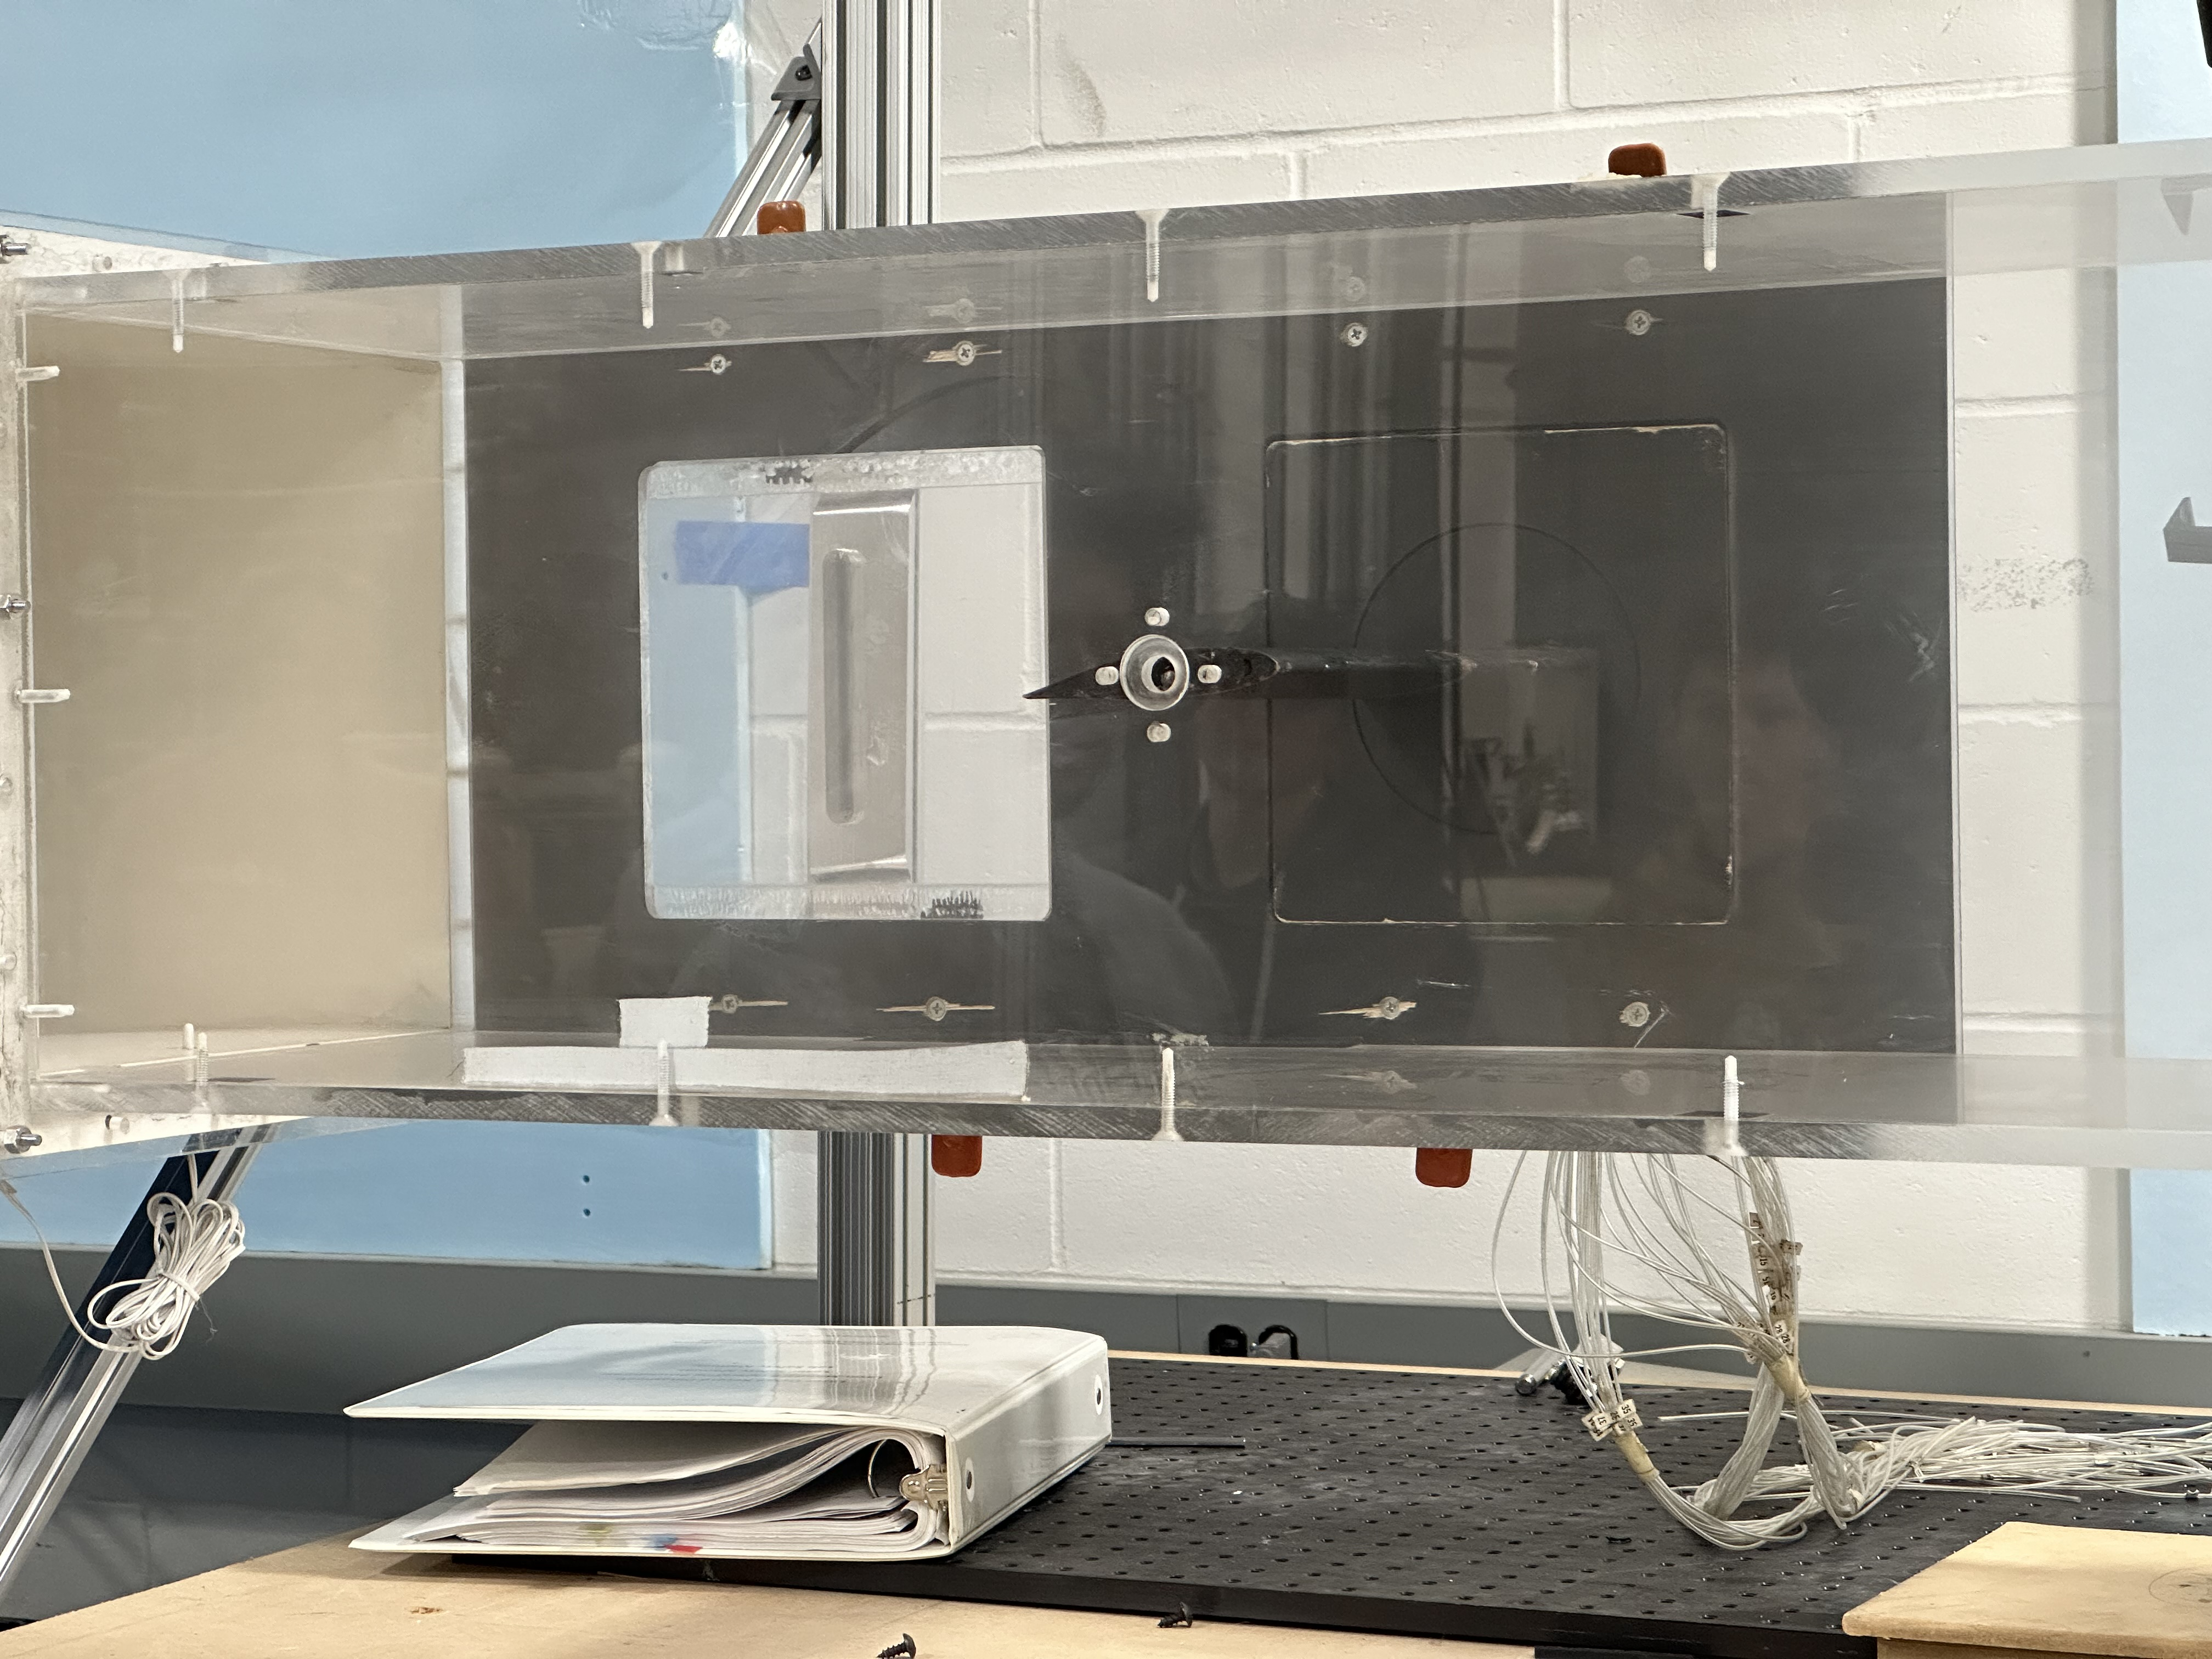
\includegraphics[width=0.75\linewidth]{Figures/IMG_0127.jpeg}
    \caption{The test section before the tests.}
    \label{fig:Test_Section}
\end{figure}

\begin{figure}[htpb]
    \centering
    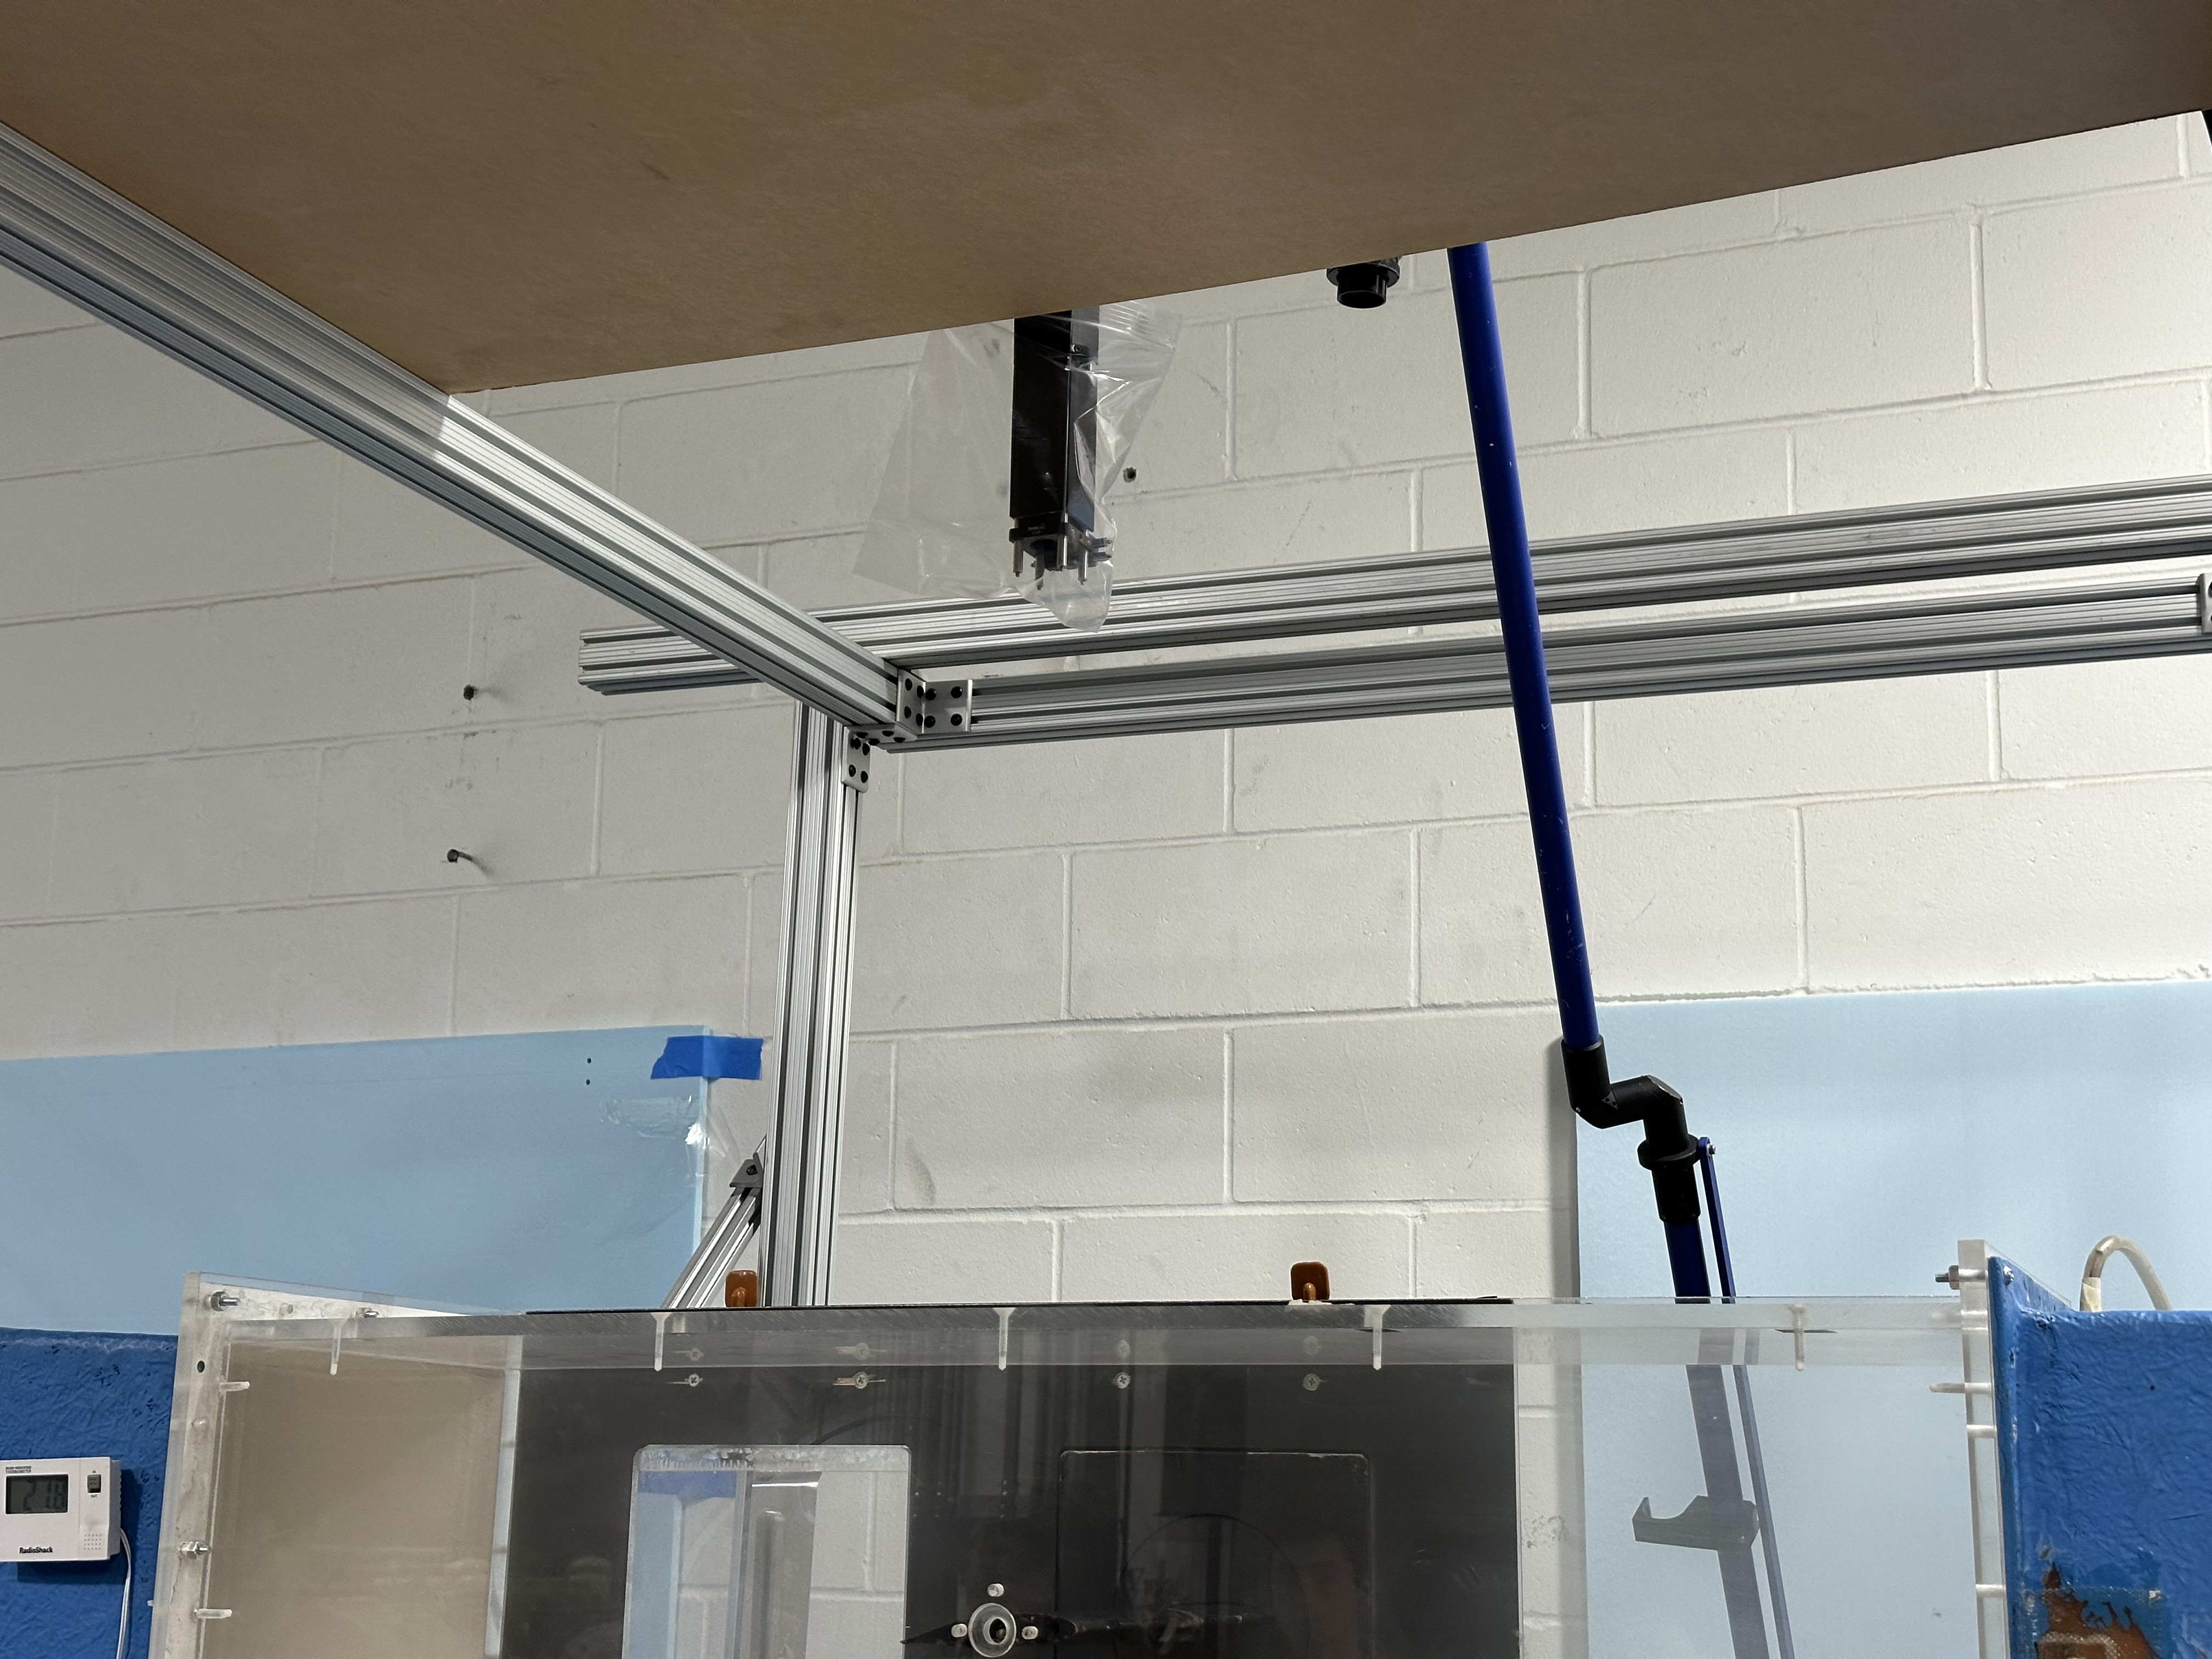
\includegraphics[width=0.75\linewidth]{Figures/IMG_0130.jpeg}
    \caption{Laser above the test section,}
    \label{fig:Laser}
\end{figure}


\begin{figure}[htpb]
    \centering
    \includegraphics[width=0.75\linewidth]{Figures/IMG_0129.jpeg}
    \caption{The mini high-speed camera.}
    \label{fig:High_Speed_Camera}
\end{figure}


\begin{figure}[htpb]
    \centering
    \includegraphics[width=0.75\linewidth]{Figures/IMG_0131.jpeg}
    \caption{Full View of Apparatus}
    \label{fig:Full_Apparatus}
\end{figure}

\section{Procedure} \label{sec:Prodedure}

\begin{enumerate}
\item Set the wind tunnel to 10 $m/s$.
\item Set the \acrshort{aoa} to 4 degrees.
\item Set up the system as described in \autoref{sec:Apparatus}.
\item Start recording data using the data collection software.
\item Repeat steps 1-4 for 8, 12, and 16 degrees.
\end{enumerate}

\section{Derivations} \label{sec: Derivations}
The PIV Data consists of x and y positions with corresponding x and y velocity. From the velocity data at each point, vorticity is found using \autoref{eq:vorticity}. This is computed using the \textit{curl} function in Matlab as the $k$ component of the velocity vector is zero and the result is the same.
\begin{equation}\label{eq:vorticity}
    \omega _z = \frac{\delta V}{\delta x} - \frac{\delta U}{\delta y}
\end{equation}
\begin{equation}\label{eq:curl}
    \Delta \times Velocity = \begin{bmatrix} i & j & k \\ \frac{\delta}{\delta x} & \frac{\delta}{\delta y} & \frac{\delta}{\delta z} \\ U & V & W \end{bmatrix} = \begin{bmatrix} i & j & k \\ \frac{\delta}{\delta x} & \frac{\delta}{\delta y} & 0 \\ U & V & 0 \end{bmatrix} = (0,0,\frac{\delta V}{\delta x} - \frac{\delta U}{\delta y})
\end{equation}
Data at every position over $N$ frames is averaged to get the mean velocity components in the x and y directions (\autoref{eq:mean_velocity}). 
\begin{equation}\label{eq:mean_velocity}
    U = \sum^N_{i=1} \frac{u_i}{N}, V = \sum^N_{i=1} \frac{v_i}{N} 
\end{equation}
From the mean velocities, the turbulent velocity fluctuations are computed at each position (\autoref{eq:fluctuation}).
\begin{equation}\label{eq:fluctuation}
    \overline{u}' = \sqrt{\sum^N_{i=1}(u_i-U)^2/N},
    \overline{v}' = \sqrt{\sum^N_{i=1}(v_i-U)^2/N}
\end{equation}
Finally, the turbulent velocity fluctuations are used to find the turbulent kinetic energy distribution, as shown in \autoref{eq:kinetic}.
\begin{equation}\label{eq:kinetic}
    TKE = \frac{1}{2}\rho(\overline{u}'^2 + \overline{v}'^2)
\end{equation}

